% Created 2021-01-05 Tue 22:34
% Intended LaTeX compiler: xelatex
\documentclass{homework}
        

\class{CS 3141: Prof. Kamil's Algorithm Analysis}
\address{Bayt El-Hikmah}
\author{Musa Al`Khwarizmi}
\date{\today}
\title{Homework in Org-mode}
\hypersetup{
 pdfauthor={Musa Al`Khwarizmi},
 pdftitle={Homework in Org-mode},
 pdfkeywords={},
 pdfsubject={},
 pdfcreator={Emacs 26.3 (Org mode 9.4)}, 
 pdflang={English}}
\begin{document}

\maketitle

\question What is this document?
\label{sec:org52d976a}

This is a demonstration of my homework \LaTeX{} class. It is an extension of the \texttt{amsart} and should have all of its functionality. These are some of the set symbols: \(\C \supset \R \supset \Q \supset \Z \supset \N \supset \F\), then some Greek and other mathematical symbols are, \(\al, \ep, \p, \ra, \Ra, \injective, \surjective, \bijective\). We can also insert multiple figures as seen in figure \ref{fig:org61ffa11}. There is also an \texttt{org-mode} version of this file\footnote{Tashfeen's \texttt{org-mode} configurations can be found \href{https://github.com/simurgh9/emacs786}{here}.}.

\begin{figure}[htbp]
\centering
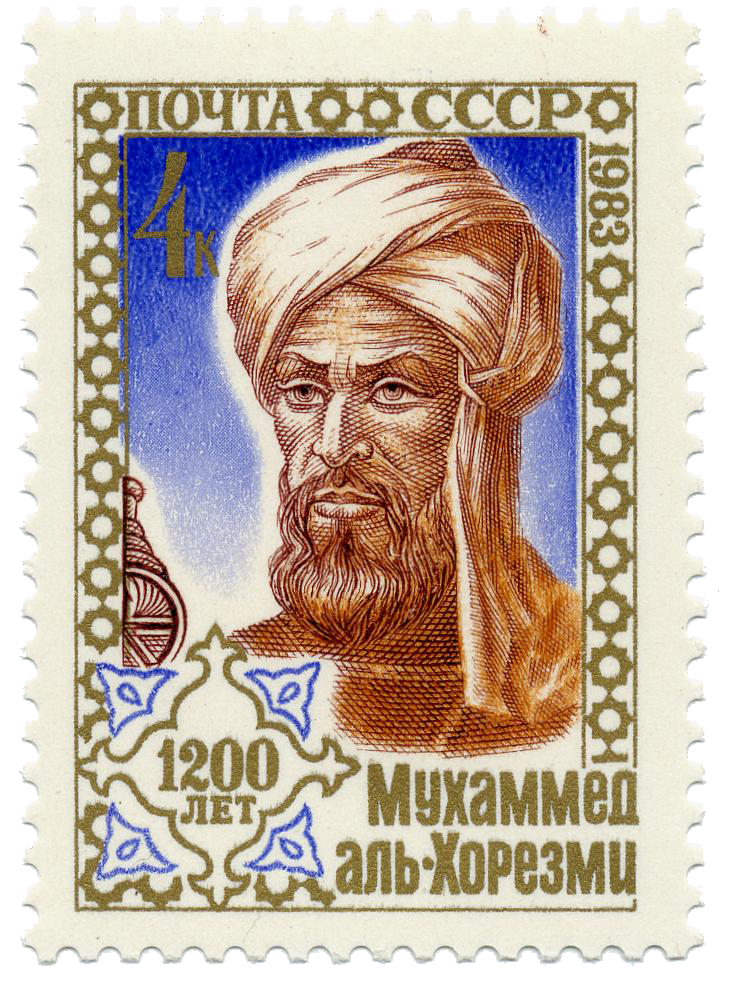
\includegraphics[width=0.2\textwidth]{../../media/khwarizmi.png}
\caption{\label{fig:org61ffa11}Al`Khwarizmi}
\end{figure}

\question Prove that square root of two is irrational.
\label{sec:org0ec0cfc}

We show,
\begin{proof}[Proof by Contradiction]
Square root of two is irrational, \(\sqrt{2} \not\in \Q\).

Assume that \(\sqrt{2}\) is rational. Then \(\sqrt{2} = p/q\) for some integers \(p,q\) with no common factors. Then \(2q^2 = p^2\) so \(p\) is even. I. e., \(p=2k\) for some \(k\). Then \(q^2=2k^2\), so \(q\) is also even which is a contradiction.
\end{proof}

\question What is the cardinality of Natural Numbers?
\label{sec:org4db6b29}
\label{orgadc0224}

It is \(\aleph_0\) \cite{arlinghaus1996part}. See also question \ref{org6cf4621}.

\question [IV] Is the cardinality of Naturals and Reals the same because they are both infinite?
\label{sec:org3b68e58}
\label{org6cf4621}

No, the cardinality of Reals is greater because they are also un-listable (uncountable). See also question \ref{orgadc0224}.

\question Finally the numbered bullets are done with the \texttt{enumitem} package,
\label{sec:orgb8dad70}

\begin{enumerate}
\item With just bullets,
\begin{itemize}
\item \textbf{Cats}
\item \emph{Dogs}
\end{itemize}
\end{enumerate}

\question [1 (Bonus)] State chain rule.
\label{sec:orgd736884}

Chain Rule:
\[
\zeta(x) = f(g(x)) \quad \text{ then according to the chain rule: } \quad
\derivative{\zeta} = \derivative[g]{f} \times \derivative{g}
\]

\question [2 (Bonus)] Euclidean Algorithm
\label{sec:orgf81143a}

You may write code as in listing,

\lstinputlisting[language=python, label=gcd, caption=Euclidean Algorithm for Greatest Common Factor]{../../media/sample.py}

\question How do we insert in-file code?
\label{sec:org318e130}

Like in listing \ref{org1a39eaf},

\lstset{language=Python,label=org1a39eaf,caption={Recursive Python function to calculate \(n^{th}\) Fibonacci number.},captionpos=b,numbers=none,numbers=left}
\begin{lstlisting}
def fib(n):
  if n == 0: return 0
  if n == 1: return 1
  return fib(n - 1) + fib(n - 2)
print(fib(20))
\end{lstlisting}


\bibliographystyle{plain}
\bibliography{../latex/citations}
\end{document}